\section{Experiments}\label{sec:exp}

This section reports the experimental configurations and results for the TTF return series. It covers the properties of the realized series alongside the ForGAN baseline across different training lengths, capacities, condition windows and input scaling. Next, the section examines the effect of cost function terms, followed by model selection and option prices. All configurations are trained with five fixed seeds, and the values are reported as mean and seed spread. The seed range of a value is its mean plus or minus one seed spread. The difference between configurations is treated as separable if their seed ranges do not overlap. A generated value is treated as separable from the test split if its seed range does not contain the realized value. Each subsection reports a defined slice of the full experimental grid from App.~\ref{app:grid}.

\subsection{Properties of the TTF Return Series}\label{sec:properties-ttf}
The daily log returns over the full sample are shown in Fig.~\ref{fig:ttf-log-returns}. The three data splits of Sec.~\ref{sec:data-split} are marked.

\begin{figure}[htbp]
    \centering
    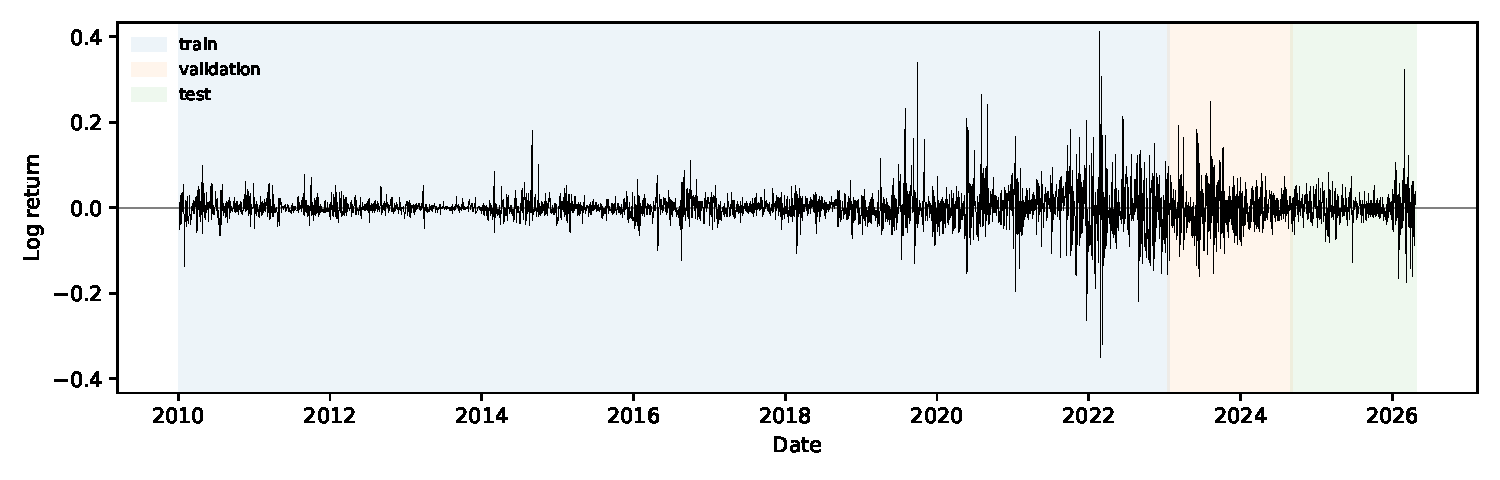
\includegraphics[width=\textwidth]{figures/ttf_log_returns.pdf}
    \caption{Daily TTF log returns with the train, validation and test splits}
    \label{fig:ttf-log-returns}
\end{figure}

Table~\ref{tab:ttf-stats} reports the distributional properties of the TTF return series, full sample and per data split. These statistics are the reference values against which generated returns are compared in the following sections. 

\begin{table}[htbp]
\centering
\begin{tabular}{lrrrr}
\toprule
 & Full & Train & Validation & Test \\
\midrule
$n$                    & 3{,}997  & 3{,}197  & 399      & 401    \\
Mean                   &  0.0003  &  0.0005  & $-$0.0014 &  0.0006  \\
Standard deviation     &  0.0395  &  0.0377  &  0.0515  &  0.0401  \\
Skewness               &  0.70    &  0.71    &  0.59    &  0.91    \\
Excess kurtosis        & 14.91    & 19.08    &  2.53    & 13.24    \\
Minimum                & $-$0.3524 & $-$0.3524 & $-$0.1615 & $-$0.1749 \\
Maximum                &  0.4128  &  0.4128  &  0.2483  &  0.3229  \\
$1\%$ quantile         & $-$0.1153 & $-$0.1129 & $-$0.1248 & $-$0.1291 \\
$99\%$ quantile        &  0.1239  &  0.1224  &  0.1639  &  0.0885  \\
$P(|x| > 0.05)$        &  0.117   &  0.099   &  0.253   &  0.130   \\
$P(|x| > 0.10)$        &  0.030   &  0.027   &  0.058   &  0.025   \\
\midrule
$C(1)$                 &  0.033   &  0.067   & $-$0.096 &  0.008   \\
$C_2(1)$               &  0.364   &  0.392   &  0.128   &  0.288   \\
$C_2(2)$               &  0.280   &  0.310   &  0.206   &  0.061   \\
$C_2(5)$               &  0.215   &  0.236   &  0.105   &  0.094   \\
$C_2(10)$              &  0.112   &  0.117   &  0.148   &  0.011   \\
\bottomrule
\end{tabular}
\caption{Distributional statistics and autocorrelation of daily TTF log returns, full sample and per data split}
\label{tab:ttf-stats}
\end{table}

\textbf{Heavy tails.} The excess kurtosis of the full series is \num{14.91}, compared to 0 for a normal distribution (Sec.~\ref{sec:stylized-facts}). Absolute returns exceed \SI{10}{\percent} on \SI{3}{\percent} of trading days. The heavy tails are not distributed evenly across the data splits. The training split, which contains the 2021 to 2022 crisis, has an excess kurtosis of \num{19.08}. The test split, which contains the 2026 disruption, has \num{13.24}. Both episodes are described in Sec.~\ref{sec:gas-markets}. The validation split does not contain a comparable event and has an excess kurtosis of \num{2.53}.

\textbf{Asymmetry.} The skewness of the full series is \num{0.70}, indicating that large positive returns are more likely than large negative returns (Sec.~\ref{sec:stylized-facts}). The skewness is positive for all data splits, with the training split at \num{0.71}, the validation split at \num{0.59} and the test split at \num{0.91}. As reported in Sec.~\ref{sec:m1-construction}, the transition days account for most of the positive skew. Skewness falls to \num{0.26}
when transition days are excluded. The remaining asymmetry is consistent with the supply disruptions described in
Sec.~\ref{sec:gas-markets}. Such events raise prices sharply, while no comparable mechanism lowers them. The positive skew is consistent with the right-skewed volatility smile reported for energy markets in Sec.~\ref{sec:implied-vol}.

\textbf{Volatility clustering.} The autocorrelation of returns at $\tau=1$, Eq.~\eqref{eq:autocorrelation}, is \num{0.033} and stays close to 0 across all data splits. The autocorrelation of squared returns, Eq.~\eqref{eq:vol-clustering}, is \num{0.364} at $\tau=1$, and decays slowly, to \num{0.280} at $\tau=2$, \num{0.215} at $\tau=5$ and \num{0.112} at $\tau=10$. The slow decay is the volatility clustering described in Sec.~\ref{sec:stylized-facts}.
The training split decays smoothly as well, while the validation and
test splits do not.
In the validation split the autocorrelation rises from \num{0.128} at $\tau=1$ to \num{0.206} at $\tau=2$, falls to \num{0.105} at $\tau=5$ and rises again to \num{0.148} at $\tau=10$. In the test split it drops from \num{0.288} to \num{0.061} between $\tau=1$ and $\tau=2$, rises to \num{0.094} at $\tau=5$ and falls to \num{0.011} at $\tau=10$. The training split holds \num{3197} of the \num{3997} observations, so the decay of the full sample follows from the training split.

The heavy tails and the volatility clustering of the test split originate in the 2026 disruption described in Sec.~\ref{sec:gas-markets}. The test split is further examined with that period removed. Table~\ref{tab:test-spike} reports the distributional properties of the full test split and the test split excluding the period from 2026-02-01 to 2026-04-30. The excluded period covers \num{57} of the \num{401} trading days.


\begin{table}[htbp]
\centering
\begin{tabular}{lrr}
\toprule
 & Test & Test excluding 2026 disruption \\
\midrule
$n$                & 401     & 344 \\
Standard deviation &  0.0401 &  0.0288 \\
Skewness           &  0.91   & $-$0.06 \\
Excess kurtosis    & 13.24   &  1.57 \\
$P(|x| > 0.10)$    &  0.025  &  0.006 \\
$C_2(1)$           &  0.288  &  0.042 \\
\bottomrule
\end{tabular}
\caption{Test split statistics with and without the 2026 disruption}
\label{tab:test-spike}
\end{table}
When the 2026 disruption is excluded, the test split does not show heavy tails, asymmetry or volatility clustering. The validation split has the highest standard deviation of all splits, and contains no comparable single event. The returns of the validation split are uniformly large, while the returns of the test split are moderate outside a single episode. 
The tails of the return distribution determine the value of out-of-the-money options (Sec.~\ref{sec:stylized-facts}). 
The excess kurtosis is \num{13.24} in the test split and \num{2.53} in the validation split. For this reason, the generated returns are compared with the test split in the following sections. The model selection of Sec.~\ref{sec:model-selection} is based on it as well. The consequence of this choice is discussed in Sec.~\ref{sec:limitations}.
\subsection{Baseline and Training Length}\label{sec:baseline}
The generated returns of the ForGAN baseline are reported for the first two configurations of Table~\ref{tab:configurations}, which differ only in their training schedule. They are compared to the statistical properties of the test split from Sec.~\ref{sec:properties-ttf}. Table~\ref{tab:baseline_training_length} reports both configurations alongside the test split. The reference values were computed from the rows of the test window matrix. With $l = 10$, the 401 returns of the test split give $n_{\mathrm{cond}} = 391$ rows. Mode collapse (Sec.~\ref{sec:evaluation}) was not detected in any run of the experimental grid.

\begin{table}[htbp]
  \centering
  \begin{tabular*}{\textwidth}{@{\extracolsep{\fill}}lrrr@{}}
    \toprule
     & Test & Configuration 1 & Configuration 2 \\
    \midrule
    Mean               & $0.0006$  & \ms{-0.0003}{0.0019} & \ms{-0.0029}{0.0019} \\
    Standard deviation & $0.0404$  & \ms{0.0303}{0.0118}  & \ms{0.0365}{0.0034}  \\
    Skewness           & $0.92$    & \ms{-0.18}{0.39}     & \ms{0.19}{0.58}      \\
    Excess kurtosis    & $13.27$   & \ms{0.32}{0.42}      & \ms{4.51}{1.52}      \\
    Minimum            & $-0.1749$ & \ms{-0.1533}{0.0474} & \ms{-0.2234}{0.0287} \\
    Maximum            & $0.3229$  & \ms{0.1357}{0.0519}  & \ms{0.2516}{0.0761}  \\
    $1\%$ quantile     & $-0.1305$ & \ms{-0.0739}{0.0251} & \ms{-0.1074}{0.0162} \\
    $99\%$ quantile    & $0.0903$  & \ms{0.0684}{0.0272}  & \ms{0.1103}{0.0163}  \\
    $P(|x| > 0.05)$    & $0.130$   & \ms{0.115}{0.124}    & \ms{0.129}{0.021}    \\
    $P(|x| > 0.10)$    & $0.026$   & \ms{0.008}{0.016}    & \ms{0.026}{0.008}    \\
    \midrule
    $C_2(1)$           & $0.289$   & \ms{-0.015}{0.056}   & \ms{0.125}{0.087}    \\
    $C_2(2)$           & $0.061$   & \ms{-0.009}{0.036}   & \ms{0.129}{0.055}    \\
    $C_2(5)$           & $0.094$   & \ms{-0.009}{0.035}   & \ms{0.164}{0.107}    \\
    $C_2(10)$          & $0.012$   & \ms{0.018}{0.032}    & \ms{0.073}{0.056}    \\
    \bottomrule
  \end{tabular*}
  \caption{Distributional statistics and autocorrelation of generated
  daily TTF log returns on the test split, ForGAN baseline, configurations 1 and 2}
  \label{tab:baseline_training_length}
\end{table}

\textbf{Heavy tails.} The excess kurtosis of the ForGAN baseline under configuration 1 is \ms{0.32}{0.42}, compared to $13.27$ for the test split. Under configuration 2, the excess kurtosis increases to \ms{4.51}{1.52}, roughly a third of the test split value. The seed spread is large; however, the ranges of the two configurations do not overlap.
The exceedance fractions of configuration 1 do not carry a reliable signal, as the seed spread is larger than the mean, \ms{0.115}{0.124} for $P(|x| > 0.05)$. Under configuration 2 both exceedance fractions match the values of the test split, \ms{0.129}{0.021} against $0.130$ and \ms{0.026}{0.008} against $0.026$. The ForGAN baseline under configuration 2 generates large returns at the observed frequency, but does not generate the few extreme returns that increase the excess kurtosis. 
The standard deviation of the ForGAN baseline under configuration 1 is \ms{0.0303}{0.0118}, compared to $0.0404$ for the test split. Under configuration 2, the standard deviation is \ms{0.0365}{0.0034}, slightly below the test split value.
Longer training increases the tail weight, but the excess kurtosis remains far below the test split. 

\textbf{Asymmetry.} The skewness of the ForGAN baseline under configuration 1 is \ms{-0.18}{0.39}, negative where the test split is positive at $0.92$. Under configuration 2, the skewness is \ms{0.19}{0.58}, roughly a fifth of the test split value. For both configurations, the seed spread crosses zero, and the ranges of the two configurations overlap. As a result, the two configurations cannot be separated based on skewness, unlike the excess kurtosis.
The minimum and maximum values provide additional information about the asymmetry. Under configuration 2 the minimum is \ms{-0.2234}{0.0287} and the maximum is \ms{0.2516}{0.0761}, against $-0.1749$ and $0.3229$ of the test split. The generated distribution extends further downward and less far upward than the test split. Neither configuration of the ForGAN baseline reproduces the skewness of the test split. 

\textbf{Volatility clustering.} The autocorrelation of the ForGAN baseline under configuration 1 is \ms{-0.015}{0.056} for $\tau=1$, compared to $0.289$ for the test split. Therefore, the generated series shows no volatility clustering. Under configuration 2 the autocorrelation is \ms{0.125}{0.087} for $\tau=1$, roughly half of the test split value, indicating some volatility clustering. At $\tau=2, 5, 10$ the autocorrelation under configuration 2 exceeds the test split, resulting in a flat autocorrelation. The generated series does not reproduce the autocorrelation decay described in Sec.~\ref{sec:stylized-facts}. The test split provides a limited reference for the shape of the decay, since its autocorrelation does not decay smoothly either (Sec.~\ref{sec:properties-ttf}).

Table~\ref{tab:mse_training_length} reports the same statistics for the MSE branch, the supervised counterpart of the ForGAN baseline, under configurations 1 and 2. The excess kurtosis of the MSE branch under configuration 1 is \ms{0.19}{0.23}, against \ms{0.32}{0.42} for the ForGAN baseline. Under configuration 2, the excess kurtosis of the MSE branch is \ms{4.13}{1.20}, close to the \ms{4.51}{1.52} of the ForGAN baseline. The two branches show similar patterns in the distributional properties.
The main difference between these two branches is the skewness. The skewness of the MSE branch under configuration 2 is \ms{0.39}{0.27}, compared to \ms{0.19}{0.58} for the ForGAN baseline. The seed spread for MSE does not cross zero, so the MSE branch reproduces a positive skew, unlike the ForGAN baseline. However, the skewness under both configurations is still below the test split value of $0.92$. The MSE branch also varies less across seeds than the ForGAN baseline on the distributional statistics, under both configurations.

\begin{table}[htbp]
  \centering
  \begin{tabular*}{\textwidth}{@{\extracolsep{\fill}}lrrr@{}}
    \toprule
     & Test & Configuration 1 & Configuration 2 \\
    \midrule
    Mean               & $0.0006$  & \ms{0.0025}{0.0026}  & \ms{-0.0011}{0.0020} \\
    Standard deviation & $0.0404$  & \ms{0.0294}{0.0095}  & \ms{0.0354}{0.0011}  \\
    Skewness           & $0.92$    & \ms{-0.07}{0.24}     & \ms{0.39}{0.27}      \\
    Excess kurtosis    & $13.27$   & \ms{0.19}{0.23}      & \ms{4.13}{1.20}      \\
    Minimum            & $-0.1749$ & \ms{-0.1349}{0.0300} & \ms{-0.2151}{0.0396} \\
    Maximum            & $0.3229$  & \ms{0.1387}{0.0513}  & \ms{0.2592}{0.0469}  \\
    $1\%$ quantile     & $-0.1305$ & \ms{-0.0674}{0.0175} & \ms{-0.0976}{0.0083} \\
    $99\%$ quantile    & $0.0903$  & \ms{0.0709}{0.0248}  & \ms{0.1114}{0.0066}  \\
    $P(|x| > 0.05)$    & $0.130$   & \ms{0.103}{0.102}    & \ms{0.124}{0.006}    \\
    $P(|x| > 0.10)$    & $0.026$   & \ms{0.005}{0.010}    & \ms{0.024}{0.002}    \\
    \midrule
    $C_2(1)$           & $0.289$   & \ms{0.040}{0.074}    & \ms{0.149}{0.063}    \\
    $C_2(2)$           & $0.061$   & \ms{0.009}{0.056}    & \ms{0.141}{0.093}    \\
    $C_2(5)$           & $0.094$   & \ms{0.007}{0.055}    & \ms{0.152}{0.088}    \\
    $C_2(10)$          & $0.012$   & \ms{0.024}{0.041}    & \ms{0.134}{0.078}    \\
    \bottomrule
  \end{tabular*}
  \caption{Distributional statistics and autocorrelation of generated
  daily TTF log returns on the test split, MSE branch, configurations 1 and 2}
  \label{tab:mse_training_length}
\end{table}

Configuration 1, corresponding to Algorithm 1 of \textcite{vuleticFinGANForecastingClassifying2024}, leaves the model undertrained on the TTF futures dataset. The generated distribution is close to a normal distribution and shows no volatility clustering.
Configuration 2, corresponding to the published implementation of \textcite{vuleticFinGANForecastingClassifying2024}, is a usable base configuration for training on the TTF futures dataset. However, the excess kurtosis and skewness remain well below the test split values.
The two branches respond to the schedule in the same way, so the difference between the two configurations is a result of the training length and not the objective.
\subsection{Network Capacity}\label{sec:network-capacity}

The generated returns for the ForGAN baseline are reported in Tables~\ref{tab:capacity_n8} and~\ref{tab:capacity_n32}. The six configurations from Table~\ref{tab:configurations} differ in the noise dimension $N$ and the LSTM hidden sizes $R_G$ and $R_D$. All six configurations follow the training length of configuration 2, so that the effect of capacity is isolated from the training schedule. Configuration 2, examined in Sec.~\ref{sec:baseline}, is carried over for reference. Table~\ref{tab:capacity_n8} holds the noise dimension at $N = 8$, and Table~\ref{tab:capacity_n32} at $N = 32$. In Table~\ref{tab:capacity_n8}, configurations 2 and 4 differ only in $R_D$, while configurations 4 and 10 differ only in $R_G$. In Table~\ref{tab:capacity_n32}, configurations 3 and 5 differ only in $R_D$, while configurations 5 and 8 differ only in $R_G$. Comparing corresponding columns across the two tables isolates $N$.


\begin{table}[htbp]
  \centering
  \begin{tabular*}{\textwidth}{@{\extracolsep{\fill}}lrrrr@{}}
    \toprule
     & Test & Configuration 2 & Configuration 4 & Configuration 10 \\
    \midrule
    Mean               & $0.0006$  & \ms{-0.0029}{0.0019} & \ms{-0.0002}{0.0014} & \ms{0.0025}{0.0022}  \\
    Standard deviation & $0.0404$  & \ms{0.0365}{0.0034}  & \ms{0.0369}{0.0029}  & \ms{0.0368}{0.0022}  \\
    Skewness           & $0.92$    & \ms{0.19}{0.58}      & \ms{-0.09}{0.38}     & \ms{-0.14}{0.61}     \\
    Excess kurtosis    & $13.27$   & \ms{4.51}{1.52}      & \ms{7.95}{1.68}      & \ms{7.85}{3.39}      \\
    Minimum            & $-0.1749$ & \ms{-0.2234}{0.0287} & \ms{-0.3212}{0.0454} & \ms{-0.2772}{0.0539} \\
    Maximum            & $0.3229$  & \ms{0.2516}{0.0761}  & \ms{0.3254}{0.0532}  & \ms{0.2850}{0.0803}  \\
    $1\%$ quantile     & $-0.1305$ & \ms{-0.1074}{0.0162} & \ms{-0.1228}{0.0128} & \ms{-0.1160}{0.0179} \\
    $99\%$ quantile    & $0.0903$  & \ms{0.1103}{0.0163}  & \ms{0.1177}{0.0184}  & \ms{0.1131}{0.0106}  \\
    $P(|x| > 0.05)$    & $0.130$   & \ms{0.129}{0.021}    & \ms{0.120}{0.012}    & \ms{0.112}{0.015}    \\
    $P(|x| > 0.10)$    & $0.026$   & \ms{0.026}{0.008}    & \ms{0.033}{0.010}    & \ms{0.027}{0.005}    \\
    \midrule
    $C_2(1)$           & $0.289$   & \ms{0.125}{0.087}    & \ms{0.057}{0.071}    & \ms{0.206}{0.086}    \\
    $C_2(2)$           & $0.061$   & \ms{0.129}{0.055}    & \ms{0.123}{0.124}    & \ms{0.310}{0.174}    \\
    $C_2(5)$           & $0.094$   & \ms{0.164}{0.107}    & \ms{0.120}{0.092}    & \ms{0.223}{0.147}    \\
    $C_2(10)$          & $0.012$   & \ms{0.073}{0.056}    & \ms{0.079}{0.038}    & \ms{0.057}{0.045}    \\
    \bottomrule
  \end{tabular*}
  \caption{Distributional statistics and autocorrelation of generated
  daily TTF log returns on the test split, ForGAN baseline, configurations 2, 4, and 10}
  \label{tab:capacity_n8}
\end{table}

\begin{table}[htbp]
  \centering
  \begin{tabular*}{\textwidth}{@{\extracolsep{\fill}}lrrrr@{}}
    \toprule
     & Test & Configuration 3 & Configuration 5 & Configuration 8 \\
    \midrule
    Mean               & $0.0006$  & \ms{-0.0016}{0.0029} & \ms{0.0001}{0.0018}  & \ms{0.0019}{0.0034}  \\
    Standard deviation & $0.0404$  & \ms{0.0353}{0.0035}  & \ms{0.0354}{0.0031}  & \ms{0.0369}{0.0036}  \\
    Skewness           & $0.92$    & \ms{0.02}{0.68}      & \ms{0.41}{0.68}      & \ms{0.54}{0.88}      \\
    Excess kurtosis    & $13.27$   & \ms{4.70}{1.53}      & \ms{7.04}{1.83}      & \ms{10.12}{2.59}     \\
    Minimum            & $-0.1749$ & \ms{-0.2326}{0.0675} & \ms{-0.2746}{0.0978} & \ms{-0.2509}{0.0482} \\
    Maximum            & $0.3229$  & \ms{0.2478}{0.0444}  & \ms{0.3497}{0.0556}  & \ms{0.3742}{0.0535}  \\
    $1\%$ quantile     & $-0.1305$ & \ms{-0.1013}{0.0213} & \ms{-0.1007}{0.0247} & \ms{-0.1055}{0.0304} \\
    $99\%$ quantile    & $0.0903$  & \ms{0.1020}{0.0167}  & \ms{0.1130}{0.0101}  & \ms{0.1185}{0.0258}  \\
    $P(|x| > 0.05)$    & $0.130$   & \ms{0.121}{0.022}    & \ms{0.110}{0.015}    & \ms{0.104}{0.016}    \\
    $P(|x| > 0.10)$    & $0.026$   & \ms{0.021}{0.007}    & \ms{0.025}{0.009}    & \ms{0.027}{0.006}    \\
    \midrule
    $C_2(1)$           & $0.289$   & \ms{0.159}{0.097}    & \ms{0.121}{0.111}    & \ms{0.263}{0.201}    \\
    $C_2(2)$           & $0.061$   & \ms{0.121}{0.028}    & \ms{0.116}{0.099}    & \ms{0.170}{0.113}    \\
    $C_2(5)$           & $0.094$   & \ms{0.105}{0.098}    & \ms{0.132}{0.127}    & \ms{0.167}{0.112}    \\
    $C_2(10)$          & $0.012$   & \ms{0.074}{0.035}    & \ms{0.043}{0.033}    & \ms{0.144}{0.103}    \\
    \bottomrule
  \end{tabular*}
  \caption{Distributional statistics and autocorrelation of generated
  daily TTF log returns on the test split, ForGAN baseline, configurations 3, 5, and 8.}
  \label{tab:capacity_n32}
\end{table}

\textbf{Discriminator hidden size.} At both values of the noise dimension $N$, the discriminator hidden size $R_D$ has a consistent effect on the excess kurtosis of the generated returns. Increasing $R_D$ from 8 to 64 raises the excess kurtosis from \ms{4.51}{1.52} under configuration 2 to \ms{7.95}{1.68} under configuration 4 at $N = 8$, and the seed ranges of the two configurations do not overlap. At $N=32$, the excess kurtosis rises from \ms{4.70}{1.53} under configuration 3 to \ms{7.04}{1.83} under configuration 5, where the seed ranges of the two configurations overlap. Both values remain below the $13.27$ of the test split. Increasing $R_D$ also affects the largest negative returns. The minimum of the generated returns reaches \ms{-0.3212}{0.0454} under configuration 4, while the minimum of the test split is $-0.1749$. The \SI{1}{\percent} quantile, however, moves from \ms{-0.1074}{0.0162} to \ms{-0.1228}{0.0128} with overlapping seed ranges. Both of these values remain above the \SI{1}{\percent} quantile of the test split, $-0.1305$. As a result, increasing $R_D$ lowers the minimum of the generated returns, while the level below which \SI{1}{\percent} of the returns fall is not separable from the seed variation.

\textbf{Generator hidden size.} The generator hidden size $R_G$ has no separable effect on the excess kurtosis of the generated returns at either noise dimension.
At $N=8$, increasing $R_G$ from 8 to 64 changes the excess kurtosis from \ms{7.95}{1.68} under configuration 4 to \ms{7.85}{3.39} under configuration 10. The seed spread doubles, from $1.68$ to $3.39$, so the larger generator makes the training less stable without changing the mean. At $N=32$, increasing $R_G$ from 8 to 64 raises the excess kurtosis from \ms{7.04}{1.83} under configuration 5 to \ms{10.12}{2.59} under configuration 8. However, the seed ranges of the two configurations overlap.
As noted in Sec.~\ref{sec:configurations}, $R_G$ is not varied in \textcite{vuleticFinGANForecastingClassifying2024} or in the published implementation, so this comparison has no counterpart in the equity results.

\textbf{Noise dimension.} The noise dimension $N$ has no separable effect on the excess kurtosis at any of the three hidden size combinations. At $R_G = R_D = 8$, increasing $N$ from 8 to 32 changes the excess kurtosis from \ms{4.51}{1.52} under configuration 2 to \ms{4.70}{1.53} under configuration 3, with overlapping seed ranges. At $R_G = 8$ and $R_D = 64$, the excess kurtosis moves from \ms{7.95}{1.68} under configuration 4 to \ms{7.04}{1.83} under configuration 5, again with overlapping seed ranges. At $R_G = R_D = 64$, the excess kurtosis increases from \ms{7.85}{3.39} under configuration 10 to \ms{10.12}{2.59} under configuration 8, again with overlapping seed ranges.

\textbf{Configuration 8.} Configuration 8 has the highest excess kurtosis of the six configurations, \ms{10.12}{2.59}, and comes closest to the $13.27$ of the test split. The standard deviation is \ms{0.0369}{0.0036} under configuration 8, and its seed range contains the $0.0404$ of the test split. The maximum return is \ms{0.3742}{0.0535}, and its seed range contains the $0.3229$ of the test split. The probability of large returns, $P(|x|>0.10)$, is \ms{0.027}{0.006}, matching the $0.026$ for the test split. The skewness is \ms{0.54}{0.88}, against the $0.92$ of the test split, with a seed range that crosses zero. Configuration 8 does not separate from the test split on the standard deviation, the maximum or the skewness, and remains below it on the excess kurtosis.

\textbf{Volatility clustering.} None of the six configurations reproduces the decay of $C_2(\tau)$ observed in the test split. $C_2(1)$ ranges from \ms{0.057}{0.071} to \ms{0.263}{0.201} across the six configurations, against the $0.289$ of the test split. $C_2(2)$ ranges from \ms{0.116}{0.099} to \ms{0.310}{0.174}, above the $0.061$ of the test split. The values are shown in Fig.~\ref{fig:c2-capacity}. The seed spreads and the means of $C_2(\tau)$ are of the same order throughout both tables, so configurations cannot be separated from one another. As noted in Sec.~\ref{sec:baseline}, the test split is a limited reference for the shape of the decay; its own autocorrelation does not decay smoothly either. Configuration 8 is the closest to the test split at $\tau=1$, at \ms{0.263}{0.201} against $0.289$, but its $C_2(\tau)$ remains near that level at $\tau=2, 5$ and $10$.

\begin{figure}[htbp]
    \centering
    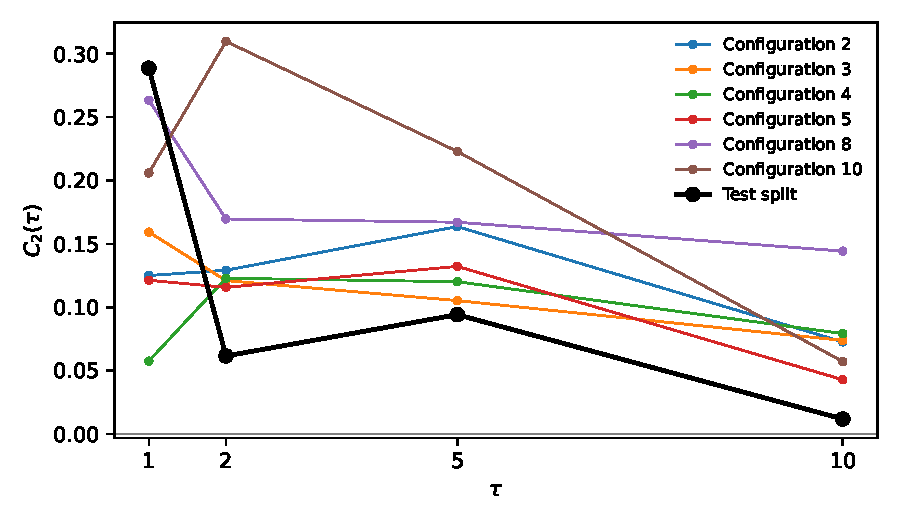
\includegraphics[width=\textwidth]{figures/c2_capacity.pdf}
    \caption{Autocorrelation of squared returns $C_2(\tau)$ for the six configurations and the test split}
    \label{fig:c2-capacity}
\end{figure}

\textbf{Training length at higher capacity.} The training length is examined further at the higher capacity settings, so the schedule of configuration 2 is no longer held fixed. Table~\ref{tab:training_length} reports the generated returns for the ForGAN baseline under configurations 7 and 9. Configurations 7 and 9 are configurations 5 and 8, respectively, with $n_{\text{epochs}} = 1500$.

The excess kurtosis of the generated returns increases from \ms{7.04}{1.83} under configuration 5 to \ms{7.97}{1.22} under configuration 7. The seed ranges overlap, so the difference in the excess kurtosis is not separable. The skewness changes from \ms{0.41}{0.68} to \ms{0.04}{0.30}, both crossing zero. The seed spreads are smaller under configuration 7 throughout the distributional statistics. As a result, a longer training schedule with a generator hidden size of $R_G = 8$ stabilizes the runs without moving them.

The excess kurtosis of the generated returns increases from \ms{10.12}{2.59} under configuration 8 to \ms{13.84}{8.77} under configuration 9. The seed ranges overlap, so the difference in the excess kurtosis is not separable. However, the mean of the excess kurtosis under configuration 9 reaches the $13.27$ of the test split. The seed spread more than triples, from $2.59$ to $8.77$, and is the largest of all configurations in this section. The skewness changes from \ms{0.54}{0.88} to \ms{1.78}{0.99}, the only skewness range among the eight configurations that does not cross zero. The skewness under configuration 9 overshoots the $0.92$ of the test split by roughly a factor of two. The maximum generated return is \ms{0.4608}{0.1127}, and its seed range excludes the $0.3229$ of the test split. $P(|x| > 0.10)$ is \ms{0.040}{0.010}, with a seed range excluding the $0.026$ of the test split. The standard deviation is \ms{0.0436}{0.0054} and its seed range contains the $0.0404$ of the test split. Configuration 9 reaches the tail weight of the test split on average and produces a reliable positive skew. However, it overshoots separably on the maximum and on $P(|x| > 0.10)$, and is the least stable of all configurations in this section.

\begin{table}[htbp]
  \centering
  \begin{tabular*}{\textwidth}{@{\extracolsep{\fill}}lrrr@{}}
    \toprule
     & Test & Configuration 7 & Configuration 9 \\
    \midrule
    Mean               & $0.0006$  & \ms{-0.0004}{0.0011} & \ms{0.0031}{0.0022}  \\
    Standard deviation & $0.0404$  & \ms{0.0368}{0.0018}  & \ms{0.0436}{0.0054}  \\
    Skewness           & $0.92$    & \ms{0.04}{0.30}      & \ms{1.78}{0.99}      \\
    Excess kurtosis    & $13.27$   & \ms{7.97}{1.22}      & \ms{13.84}{8.77}     \\
    Minimum            & $-0.1749$ & \ms{-0.3178}{0.0355} & \ms{-0.2355}{0.0246} \\
    Maximum            & $0.3229$  & \ms{0.3545}{0.0445}  & \ms{0.4608}{0.1127}  \\
    $1\%$ quantile     & $-0.1305$ & \ms{-0.1166}{0.0129} & \ms{-0.1085}{0.0082} \\
    $99\%$ quantile    & $0.0903$  & \ms{0.1163}{0.0084}  & \ms{0.1566}{0.0316}  \\
    $P(|x| > 0.05)$    & $0.130$   & \ms{0.114}{0.007}    & \ms{0.137}{0.012}    \\
    $P(|x| > 0.10)$    & $0.026$   & \ms{0.030}{0.004}    & \ms{0.040}{0.010}    \\
    \midrule
    $C_2(1)$           & $0.289$   & \ms{0.153}{0.070}    & \ms{0.160}{0.084}    \\
    $C_2(2)$           & $0.061$   & \ms{0.118}{0.088}    & \ms{0.199}{0.110}    \\
    $C_2(5)$           & $0.094$   & \ms{0.143}{0.100}    & \ms{0.115}{0.059}    \\
    $C_2(10)$          & $0.012$   & \ms{0.090}{0.058}    & \ms{0.052}{0.042}    \\
    \bottomrule
  \end{tabular*}
  \caption{Distributional statistics and autocorrelation of generated
  daily TTF log returns on the test split, ForGAN baseline, configurations 7 and 9}
  \label{tab:training_length}
\end{table}

Increasing $R_D$ from 8 to 64 is the only capacity change whose effect holds across the two tables. $R_G$ and $N$ have no separable effect on the generated returns. Of the six configurations with a fixed training schedule, configuration 8 is the closest to the test split. However, it remains below the test split on the excess kurtosis. A longer training schedule does not produce a separable change at $R_G=8$. At $R_G = 64$, a longer training schedule brings the mean of the excess kurtosis to the test split value and produces a positive skew, at the cost of stability across seeds. An increase in capacity alone does not close the gap. However, capacity combined with a longer schedule reaches the tail weight of the test split without reproducing its distribution. The condition window and the input scaling are examined in Sec.~\ref{sec:condition-window}.
\subsection{Condition Window and Input Scaling}\label{sec:condition-window}

The generated returns for the ForGAN baseline under varied condition window lengths and input scaling configurations are reported in Table~\ref{tab:condition_window} and Table~\ref{tab:scaling}, respectively. Configuration 5 is the shared baseline against which the two other configurations are compared. The full-split scaling configuration is configuration 5 with the standardization applied to the full training split rather than the reference subset of $n_{\text{batch}}=100$. Configuration 6 is configuration 5 with a longer condition window of $l=30$. With $l=30$ the 401 returns of the test split give $n_{\mathrm{cond}} = 371$ rows instead of $391$. As a result, the reference values of the test split differ in Table~\ref{tab:condition_window}, and the values of configuration 5 are reported in Table~\ref{tab:scaling}.

\begin{table}[htbp]
  \centering
  \begin{tabular}{lrr}
    \toprule
     & Test & Configuration 6 \\
    \midrule
    Mean               & $0.0003$  & \ms{-0.0006}{0.0026} \\
    Standard deviation & $0.0408$  & \ms{0.0342}{0.0019}  \\
    Skewness           & $0.96$    & \ms{0.15}{0.45}      \\
    Excess kurtosis    & $13.43$   & \ms{3.74}{1.00}      \\
    Minimum            & $-0.1749$ & \ms{-0.1893}{0.0538} \\
    Maximum            & $0.3229$  & \ms{0.2314}{0.0248}  \\
    $1\%$ quantile     & $-0.1333$ & \ms{-0.0935}{0.0062} \\
    $99\%$ quantile    & $0.0939$  & \ms{0.0930}{0.0163}  \\
    $P(|x| > 0.05)$    & $0.129$   & \ms{0.119}{0.012}    \\
    $P(|x| > 0.10)$    & $0.027$   & \ms{0.016}{0.006}    \\
    \midrule
    $C_2(1)$           & $0.288$   & \ms{0.191}{0.086}    \\
    $C_2(2)$           & $0.060$   & \ms{0.151}{0.107}    \\
    $C_2(5)$           & $0.093$   & \ms{0.125}{0.048}    \\
    $C_2(10)$          & $0.011$   & \ms{0.111}{0.107}    \\
    \bottomrule
  \end{tabular}
  \caption{Distributional statistics and autocorrelation of generated daily TTF
  log returns on the test split, ForGAN baseline, configuration 6}
  \label{tab:condition_window}
\end{table}

\textbf{Condition window.} The excess kurtosis of the ForGAN baseline decreases from \ms{7.04}{1.83} under configuration 5 to \ms{3.74}{1.00} under configuration 6, compared to the $13.43$ of the test split. The difference is separable, since the seed ranges of the two configurations do not overlap. Configurations 5 and 6 are measured against different reference values of the test split, so the comparison between them is approximate. However, the two reference values differ by $0.16$, while the excess kurtosis falls by $3.30$, so the difference in reference cannot account for the effect. The maximum return is \ms{0.2314}{0.0248} and its seed range does not include the $0.3229$ of the test split. Both exceedance fractions fall short of the test split, \ms{0.119}{0.012} against $0.129$ for $P(|x| > 0.05)$ and \ms{0.016}{0.006} against $0.027$ for $P(|x| > 0.10)$. The skewness is \ms{0.15}{0.45} and crosses zero. Configuration 6 is the furthest from the test split of the configurations trained under the schedule of configuration 2. Increasing the condition window from $l=10$ to $l=30$ reduces the tail weight of the generated returns.

\textbf{Input scaling.} The standard deviation is \ms{0.0354}{0.0031} under configuration 5 and \ms{0.0338}{0.0018} under the full-split scaling configuration, with overlapping seed ranges. The excess kurtosis decreases from \ms{7.04}{1.83} under configuration 5 to \ms{5.55}{2.52} under the full-split scaling configuration. The seed ranges of the two configurations overlap, so the difference is not separable. The skewness for the full-split scaling configuration is \ms{0.30}{0.36}, compared to \ms{0.41}{0.68} for configuration 5, and both seed ranges cross zero. Computing the scaling parameters from the full training split has no separable effect on the generated returns.

\begin{table}[htbp]
  \centering
  \begin{tabular*}{\textwidth}{@{\extracolsep{\fill}}lrrr@{}}
    \toprule
     & Test & Configuration 5 & Full-split scaling \\
    \midrule
    Mean               & $0.0006$  & \ms{0.0001}{0.0018}  & \ms{-0.0001}{0.0022} \\
    Standard deviation & $0.0404$  & \ms{0.0354}{0.0031}  & \ms{0.0338}{0.0018}  \\
    Skewness           & $0.92$    & \ms{0.41}{0.68}      & \ms{0.30}{0.36}      \\
    Excess kurtosis    & $13.27$   & \ms{7.04}{1.83}      & \ms{5.55}{2.52}      \\
    Minimum            & $-0.1749$ & \ms{-0.2746}{0.0978} & \ms{-0.2350}{0.0682} \\
    Maximum            & $0.3229$  & \ms{0.3497}{0.0556}  & \ms{0.3091}{0.0713}  \\
    $1\%$ quantile     & $-0.1305$ & \ms{-0.1007}{0.0247} & \ms{-0.0953}{0.0119} \\
    $99\%$ quantile    & $0.0903$  & \ms{0.1130}{0.0101}  & \ms{0.1002}{0.0123}  \\
    $P(|x| > 0.05)$    & $0.130$   & \ms{0.110}{0.015}    & \ms{0.109}{0.018}    \\
    $P(|x| > 0.10)$    & $0.026$   & \ms{0.025}{0.009}    & \ms{0.019}{0.006}    \\
    \midrule
    $C_2(1)$           & $0.289$   & \ms{0.121}{0.111}    & \ms{0.121}{0.121}    \\
    $C_2(2)$           & $0.061$   & \ms{0.116}{0.099}    & \ms{0.133}{0.125}    \\
    $C_2(5)$           & $0.094$   & \ms{0.132}{0.127}    & \ms{0.128}{0.135}    \\
    $C_2(10)$          & $0.012$   & \ms{0.043}{0.033}    & \ms{0.109}{0.076}    \\
    \bottomrule
  \end{tabular*}
  \caption{Distributional statistics and autocorrelation of generated daily TTF
  log returns on the test split, ForGAN baseline, configuration 5 with
  reference and full-split input scaling}
  \label{tab:scaling}
\end{table}

Configuration 6 differs separably from configuration 5 in the excess kurtosis. However, it reduces the tail weight rather than increasing it. The full-split scaling configuration shows no separable effect from configuration 5 in the standard deviation, the excess kurtosis and the skewness. Neither variation of configuration 5 improves the distributional properties of the generated returns. The effect of the cost function terms is examined in Sec.~\ref{sec:effect-cost}.


\clearpage
\subsection{Effect of the Cost Function Terms}\label{sec:effect-cost}
The generated returns for the ten cost function branches of Sec.~\ref{sec:configurations} are reported in Tables~\ref{tab:loss_c9_single}, \ref{tab:loss_c9_nosr} and~\ref{tab:loss_c9_sr}. All ten branches are trained under configuration 8 to isolate the effect of the cost function. As reported in Sec.~\ref{sec:network-capacity}, configuration 8 is the closest to the test split among the configurations that remain stable across seeds. Table~\ref{tab:loss_c9_single} reports the single cost function terms. Tables~\ref{tab:loss_c9_nosr} and~\ref{tab:loss_c9_sr} report the combinations of cost function terms, separated by the presence of the $\mathrm{SR}^{*}$ term. The ForGAN baseline is reported as a reference in all three tables. The full results for all configurations and cost function branches are given in App.~\ref{app:grid}.

\textbf{Heavy tails.} None of the nine cost function branches is separable from ForGAN on excess kurtosis, as all ten seed ranges overlap. The mean excess kurtosis of all branches is below the \num{13.27} of the test split. The lowest excess kurtosis is \ms{6.78}{1.29} for the $\mathrm{PnL}^{*}_{a}$ \& $\mathrm{MSE}$ \& $\mathrm{STD}$ branch and the highest is \ms{12.03}{5.45} for the $\mathrm{PnL}^{*}_{a}$ branch, compared to \ms{10.12}{2.59} of the ForGAN baseline and \num{13.27} of the test split. The seed ranges of the $\mathrm{MSE}$, $\mathrm{PnL}^{*}_{a}$ and $\mathrm{PnL}^{*}_{a}$ \& $\mathrm{MSE}$ branches contain the \num{13.27} of the test split, while every other branch falls short. The standard deviation is the lowest for the $\mathrm{SR}^{*}$ \& $\mathrm{MSE}$ branch at \ms{0.0331}{0.0034} and the highest for the $\mathrm{PnL}^{*}_{a}$ branch at \ms{0.0414}{0.0030}. The seed ranges of the ForGAN baseline, $\mathrm{PnL}^{*}_{a}$ and $\mathrm{PnL}^{*}_{a}$ \& $\mathrm{MSE}$ contain the \num{0.0404} of the test split, while every other branch falls short. The seed range of $P(|x|>0.10)$ is separable from ForGAN only for the $\mathrm{SR}^{*}$ \& $\mathrm{MSE}$ branch at \ms{0.016}{0.004} against \ms{0.027}{0.006}.

\begin{table}[H]
  \centering
  \small
  \setlength{\tabcolsep}{4pt}
  \begin{tabular*}{\textwidth}{l@{\extracolsep{\fill}}rrrr}
    \toprule
     & ForGAN & MSE & PnL$^*_a$ & SR$^*$ \\
    \midrule
    Mean & \msa{0.0019}{0.0034} & \msa{0.0006}{0.0023} & \msa{0.0004}{0.0030} & \msa{0.0010}{0.0005} \\
    Standard deviation & \msa{0.0369}{0.0036} & \msa{0.0377}{0.0024} & \msa{0.0414}{0.0030} & \msa{0.0341}{0.0036} \\
    Skewness & \msa{0.54}{0.88} & \msa{0.23}{1.29} & \msa{0.93}{0.30} & \msa{-0.59}{0.16} \\
    Excess kurtosis & \msa{10.12}{2.59} & \msa{10.13}{4.39} & \msa{12.03}{5.45} & \msa{8.08}{2.72} \\
    Minimum & \msa{-0.2509}{0.0482} & \msa{-0.2644}{0.0655} & \msa{-0.2542}{0.0468} & \msa{-0.2612}{0.0373} \\
    Maximum & \msa{0.3742}{0.0535} & \msa{0.3343}{0.1207} & \msa{0.3950}{0.0887} & \msa{0.2268}{0.0474} \\
    1 \% quantile & \msa{-0.1055}{0.0304} & \msa{-0.1155}{0.0144} & \msa{-0.1297}{0.0187} & \msa{-0.0913}{0.0171} \\
    99 \% quantile & \msa{0.1185}{0.0258} & \msa{0.1200}{0.0257} & \msa{0.1401}{0.0235} & \msa{0.0945}{0.0113} \\
    $P(|x| > 0.05)$ & \msa{0.104}{0.016} & \msa{0.106}{0.006} & \msa{0.119}{0.010} & \msa{0.100}{0.025} \\
    $P(|x| > 0.10)$ & \msa{0.027}{0.006} & \msa{0.030}{0.007} & \msa{0.036}{0.005} & \msa{0.017}{0.005} \\
    \midrule
    $C_2(1)$ & \msa{0.263}{0.201} & \msa{0.165}{0.122} & \msa{0.226}{0.077} & \msa{0.229}{0.039} \\
    $C_2(2)$ & \msa{0.170}{0.113} & \msa{0.181}{0.097} & \msa{0.185}{0.144} & \msa{0.377}{0.156} \\
    $C_2(5)$ & \msa{0.167}{0.112} & \msa{0.183}{0.069} & \msa{0.182}{0.072} & \msa{0.158}{0.022} \\
    $C_2(10)$ & \msa{0.144}{0.103} & \msa{0.112}{0.114} & \msa{0.153}{0.134} & \msa{0.060}{0.061} \\
    \bottomrule
  \end{tabular*}
  \caption{Distributional statistics and autocorrelation of generated daily TTF log returns on the test split, the single cost function terms, configuration 8}
  \label{tab:loss_c9_single}
\end{table}
\textbf{Asymmetry.} The seed ranges of all four branches containing the $\mathrm{SR}^{*}$ term are separable from ForGAN on skewness, and all four are negative. The skewness is \ms{-0.59}{0.16} for the $\mathrm{SR}^{*}$ branch, and the three branches containing $\mathrm{SR}^{*}$ are within \num{0.05} of it, against the \ms{0.54}{0.88} of the ForGAN baseline and the \num{0.92} of the test split.  The mean skewness of the $\mathrm{PnL}^{*}_{a}$ \& $\mathrm{STD}$ branch is \ms{-0.09}{0.95}, but its seed range crosses zero and overlaps that of the ForGAN baseline. The highest skewness is \ms{1.11}{0.42} for the $\mathrm{PnL}^{*}_{a}$ \& $\mathrm{MSE}$ \& $\mathrm{STD}$ branch. The seed ranges of the ForGAN baseline
and of the $\mathrm{MSE}$, $\mathrm{PnL}^{*}_{a}$, $\mathrm{PnL}^{*}_{a}$ \& $\mathrm{MSE}$ and $\mathrm{PnL}^{*}_{a}$ \& $\mathrm{MSE}$ \& $\mathrm{STD}$ branches contain the \num{0.92} of the test split.

The $\mathrm{SR}^{*}$ economics-driven term determines the sign of the skewness regardless of what it is combined with. The skewness is \ms{0.93}{0.30} for the $\mathrm{PnL}^{*}_{a}$ branch alone, compared to the \ms{-0.64}{0.20} of the $\mathrm{PnL}^{*}_{a}$ \& $\mathrm{SR}^{*}$ branch. As defined in Eq.~\eqref{eq:sharpe-ratio}, $\mathrm{SR}^{*}$ is the mean of the $\mathrm{PnL}^{*}_{a}$ series divided by its standard deviation. A forecast with $p_i$ far above the others increases the numerator and the denominator. As reported in Sec.~\ref{sec:properties-ttf}, large positive returns are more likely than large negative ones in the TTF series. As a result, the forecasts made on those days can decrease $\mathrm{SR}^{*}$, while they always increase $\mathrm{PnL}^{*}_{a}$.

\begin{table}[H]
  \centering
  \small
  \setlength{\tabcolsep}{4pt}
  \begin{tabular*}{\textwidth}{l@{\extracolsep{\fill}}rrrr}
    \toprule
     & ForGAN & PnL$^*_a$ \& MSE & PnL$^*_a$ \& STD & PnL$^*_a$ \& MSE \& STD \\
    \midrule
    Mean & \msa{0.0019}{0.0034} & \msa{0.0009}{0.0020} & \msa{-0.0007}{0.0032} & \msa{0.0012}{0.0009} \\
    Standard deviation & \msa{0.0369}{0.0036} & \msa{0.0397}{0.0032} & \msa{0.0356}{0.0017} & \msa{0.0353}{0.0032} \\
    Skewness & \msa{0.54}{0.88} & \msa{0.81}{0.46} & \msa{-0.09}{0.95} & \msa{1.11}{0.42} \\
    Excess kurtosis & \msa{10.12}{2.59} & \msa{10.69}{2.97} & \msa{8.21}{3.68} & \msa{6.78}{1.29} \\
    Minimum & \msa{-0.2509}{0.0482} & \msa{-0.2401}{0.0302} & \msa{-0.2821}{0.0737} & \msa{-0.1979}{0.0157} \\
    Maximum & \msa{0.3742}{0.0535} & \msa{0.3892}{0.0618} & \msa{0.3181}{0.0776} & \msa{0.3562}{0.0312} \\
    1 \% quantile & \msa{-0.1055}{0.0304} & \msa{-0.1186}{0.0200} & \msa{-0.1114}{0.0101} & \msa{-0.0882}{0.0114} \\
    99 \% quantile & \msa{0.1185}{0.0258} & \msa{0.1273}{0.0177} & \msa{0.1081}{0.0202} & \msa{0.1236}{0.0133} \\
    $P(|x| > 0.05)$ & \msa{0.104}{0.016} & \msa{0.119}{0.019} & \msa{0.109}{0.008} & \msa{0.112}{0.021} \\
    $P(|x| > 0.10)$ & \msa{0.027}{0.006} & \msa{0.032}{0.005} & \msa{0.025}{0.005} & \msa{0.025}{0.007} \\
    \midrule
    $C_2(1)$ & \msa{0.263}{0.201} & \msa{0.215}{0.049} & \msa{0.281}{0.130} & \msa{0.234}{0.122} \\
    $C_2(2)$ & \msa{0.170}{0.113} & \msa{0.183}{0.126} & \msa{0.201}{0.092} & \msa{0.124}{0.127} \\
    $C_2(5)$ & \msa{0.167}{0.112} & \msa{0.239}{0.132} & \msa{0.129}{0.041} & \msa{0.081}{0.110} \\
    $C_2(10)$ & \msa{0.144}{0.103} & \msa{0.129}{0.068} & \msa{0.125}{0.075} & \msa{0.067}{0.070} \\
    \bottomrule
  \end{tabular*}
  \caption{Distributional statistics and autocorrelation of generated daily TTF log returns on the test split, the combinations without the SR term, configuration 8}
  \label{tab:loss_c9_nosr}
\end{table}

The seed ranges of the maximum of all four branches containing $\mathrm{SR}^{*}$ are separable from the \ms{0.3742}{0.0535} of the ForGAN baseline, and all four are lower. The maximum is \ms{0.2154}{0.0369} for the $\mathrm{SR}^{*}$ \& $\mathrm{MSE}$
branch, and the other three are within \num{0.012} of it. The seed ranges of the ForGAN baseline and of the $\mathrm{MSE}$, $\mathrm{PnL}^{*}_{a}$ and $\mathrm{PnL}^{*}_{a}$ \& $\mathrm{STD}$ branches contain the \num{0.3229} of the test split. The maximum of the $\mathrm{PnL}^{*}_{a}$ \& $\mathrm{MSE}$ branch is \ms{0.3892}{0.0618}, above the test split. 
The seed ranges of the \SI{99}{\percent} quantile of all four branches containing $\mathrm{SR}^{*}$ and of the $\mathrm{PnL}^{*}_{a}$ \& $\mathrm{STD}$ branch contain the \num{0.0903} of the test split, while that of the ForGAN baseline lies above it. 
The seed ranges of the \SI{1}{\percent} quantile of the ForGAN baseline and of the $\mathrm{PnL}^{*}_{a}$ and $\mathrm{PnL}^{*}_{a}$ \& $\mathrm{MSE}$ branches contain the \num{-0.1305} of the test split.
All ten branches lie below the minimum of the test split, \num{-0.1749}. The closest is the $\mathrm{PnL}^{*}_{a}$ \& $\mathrm{MSE}$ \& $\mathrm{STD}$ branch at \ms{-0.1979}{0.0157}.

The seed ranges of the $\mathrm{PnL}^{*}_{a}$ branch contain the test split on the skewness, the maximum and the \SI{1}{\percent} quantile, as does the ForGAN baseline. $\mathrm{SR}^{*}$ compresses the largest generated return, which brings the \SI{99}{\percent} quantile closer to the test split but moves the skewness and the maximum away.

\begin{table}[H]
  \centering
  \small
  \setlength{\tabcolsep}{4pt}
  \begin{tabular*}{\textwidth}{l@{\extracolsep{\fill}}rrrr}
    \toprule
     & ForGAN & PnL$^*_a$ \& SR$^*$ & SR$^*$ \& MSE & PnL$^*_a$ \& MSE \& SR$^*$ \\
    \midrule
    Mean & \msa{0.0019}{0.0034} & \msa{0.0012}{0.0020} & \msa{0.0007}{0.0011} & \msa{0.0007}{0.0014} \\
    Standard deviation & \msa{0.0369}{0.0036} & \msa{0.0351}{0.0031} & \msa{0.0331}{0.0034} & \msa{0.0338}{0.0034} \\
    Skewness & \msa{0.54}{0.88} & \msa{-0.64}{0.20} & \msa{-0.57}{0.20} & \msa{-0.60}{0.24} \\
    Excess kurtosis & \msa{10.12}{2.59} & \msa{8.03}{2.55} & \msa{8.02}{2.42} & \msa{7.86}{2.93} \\
    Minimum & \msa{-0.2509}{0.0482} & \msa{-0.2638}{0.0303} & \msa{-0.2553}{0.0310} & \msa{-0.2570}{0.0406} \\
    Maximum & \msa{0.3742}{0.0535} & \msa{0.2207}{0.0322} & \msa{0.2154}{0.0369} & \msa{0.2231}{0.0509} \\
    1 \% quantile & \msa{-0.1055}{0.0304} & \msa{-0.0938}{0.0122} & \msa{-0.0889}{0.0153} & \msa{-0.0910}{0.0147} \\
    99 \% quantile & \msa{0.1185}{0.0258} & \msa{0.0959}{0.0122} & \msa{0.0921}{0.0089} & \msa{0.0930}{0.0088} \\
    $P(|x| > 0.05)$ & \msa{0.104}{0.016} & \msa{0.108}{0.021} & \msa{0.094}{0.022} & \msa{0.100}{0.023} \\
    $P(|x| > 0.10)$ & \msa{0.027}{0.006} & \msa{0.017}{0.006} & \msa{0.016}{0.004} & \msa{0.016}{0.005} \\
    \midrule
    $C_2(1)$ & \msa{0.263}{0.201} & \msa{0.223}{0.089} & \msa{0.202}{0.059} & \msa{0.225}{0.103} \\
    $C_2(2)$ & \msa{0.170}{0.113} & \msa{0.382}{0.146} & \msa{0.274}{0.111} & \msa{0.345}{0.134} \\
    $C_2(5)$ & \msa{0.167}{0.112} & \msa{0.163}{0.075} & \msa{0.153}{0.025} & \msa{0.147}{0.036} \\
    $C_2(10)$ & \msa{0.144}{0.103} & \msa{0.056}{0.047} & \msa{0.076}{0.061} & \msa{0.057}{0.038} \\
    \bottomrule
  \end{tabular*}
  \caption{Distributional statistics and autocorrelation of generated daily TTF log returns on the test split, the combinations with the SR term, configuration 8}
  \label{tab:loss_c9_sr}
\end{table}

\textbf{Volatility clustering.} None of the ten branches reproduces the decay of $C_2(\tau)$ observed in the test split. $C_2(1)$ ranges from \ms{0.165}{0.122} to \ms{0.281}{0.130} across the ten branches, against the $0.289$ of the test split. The seed spreads are of the same order as the means, so the branches are not separable. The four branches containing $\mathrm{SR}^{*}$ rise from $C_2(1)$ between
\num{0.202} and \num{0.229} to $C_2(2)$ between \num{0.274} and \num{0.382}, where the test split falls to $0.061$. The seed spreads of the four branches at $\tau=2$ are between \num{0.111} and \num{0.156}, so they do not separate from the other branches.

The $\mathrm{SR}^{*}$, $\mathrm{PnL}^{*}_{a}$ \& $\mathrm{SR}^{*}$,
$\mathrm{SR}^{*}$ \& $\mathrm{MSE}$ and $\mathrm{PnL}^{*}_{a}$ \& $\mathrm{MSE}$ \& $\mathrm{SR}^{*}$ are the only branches separable from ForGAN on the skewness and the maximum. The $\mathrm{PnL}^{*}_{a}$ and $\mathrm{PnL}^{*}_{a}$ \& $\mathrm{MSE}$ branches come closest to the test split overall. Their seed ranges contain the test split values on the skewness, the excess kurtosis, the standard deviation and the \SI{1}{\percent} quantile. Overall, no economics-driven term separably improves the ForGAN baseline. As described in Sec.~\ref{sec:training-config}, the economics-driven terms of \textcite{vuleticFinGANForecastingClassifying2024} target the directional accuracy of the forecast, which is not the criterion used here. The effect of the cost function on the option prices is examined in Sec.~\ref{sec:option-prices}. 

% - [ ] Close: the cost function does not affect volatility clustering,
%       consistent with Sec. 5.3 and Sec. 5.4


% ## 5.5 Effect of the Cost Function Terms — TODO
%
% Tables 12 (single terms), 13 (without SR), 14 (with SR).
% Configuration 8 throughout, ForGAN repeated as the reference column.
% Test split reference: skew 0.92, kurtosis 13.27, SD 0.0404,
% max 0.3229, min -0.1749, P(0.05) 0.130, P(0.10) 0.026,
% q99 0.0903, q01 -0.1305.
%

\subsection{Model Selection}\label{sec:model-selection}

Configuration 8 is selected for the generation of price paths,  together with the $\mathrm{PnL}^{*}_{a}$ cost function branch. As listed in Tab.~\ref{tab:configurations}, configuration 8 uses a condition window of $l=10$, a noise dimension of $N=32$, generator and discriminator hidden sizes of $R_D=R_G=64$ and $n_{\mathrm{grad}} + n_{\mathrm{epochs}} = 100 + 500$. 

\textbf{Network capacity.} Configuration 9 is closer to the test split than configuration 8 on the excess kurtosis and the skewness. Its skewness seed range is also the only one that does not cross zero. However, the seed spread of configuration 9 on the excess kurtosis is more than three times as wide as the seed spread of configuration 8. Its maximum exceeds the test split, while the seed range of configuration 8 contains it (Sec.~\ref{sec:network-capacity}). Reproducibility across seeds is taken as the selection criterion, not proximity of the mean. As a result, configuration 8 is chosen over configuration 9.

\textbf{Cost function.} No branch is separable from ForGAN, so the separability criterion cannot distinguish between them. Selection among the branches is based on closeness to the test split. As reported in Sec.~\ref{sec:effect-cost}, under configuration 8 the seed ranges of the $\mathrm{PnL}^{*}_{a}$ and $\mathrm{PnL}^{*}_{a}$ \& $\mathrm{MSE}$ branches contain the test split on the skewness, the excess kurtosis, the standard deviation and the \SI{1}{\percent} quantile. The seed range of the $\mathrm{PnL}^{*}_{a}$ branch contains the maximum of the test split. The $\mathrm{PnL}^{*}_{a}$ \& $\mathrm{MSE}$ branch exceeds it across all seeds. The seed range of the $\mathrm{PnL}^{*}_{a}$ branch is closer to the test split on the standard deviation than the ForGAN baseline, and its skewness seed range is also narrower. The $\mathrm{PnL}^{*}_{a}$ branch is chosen over the ForGAN baseline and the $\mathrm{PnL}^{*}_{a}$ \& $\mathrm{MSE}$ branch. The selected model generates the price paths of Sec.~\ref{sec:option-prices}.

% ### Closing paragraph — what the selected model does not reproduce
%
% - [ ] PURPOSE: forward-looking, not a summary. Tells the reader how to
%       read Sec. 5.7. Do not restate the two decisions
%
% - [ ] Numbers are the PnL*a column of Tab. 12, NOT ForGAN. ForGAN sits
%       immediately to its left, easy to grab the wrong one
%
% - [ ] S1. The body of the distribution is close: the seed ranges contain
%       the test split on the skewness, the excess kurtosis and the
%       standard deviation. One clause, cite Sec. 5.5, no numbers
%
% - [ ] S2. The extremes do not match. Minimum -0.2542 against the
%       -0.1749 of the test split; maximum 0.3950 against 0.3229.
%       Both overshoot
%
% - [ ] S3. The autocorrelation of squared returns does not decay:
%       C2(10) is 0.153 against the 0.011 of the test split
%
% - [ ] S4. Name the consequence for Sec. 5.7 WITHOUT stating a direction:
%       the far strikes depend on the extremes, so they are affected.
%       DO NOT say whether prices come out too high or too low — that is
%       5.7's result
%
% - [ ] Keep to four sentences. This paragraph frames 5.7, it does not
%       pre-empt it

\subsection{Option Prices}\label{sec:option-prices}

The price paths were generated with the ForGAN baseline model under configuration 8, selected in Sec.~\ref{sec:model-selection}, and priced through the procedure described in Sec.~\ref{sec:pricing-setup}. The generated option prices are evaluated against the market prices as well as the benchmarks of Sec.~\ref{sec:benchmarks}. Option prices depend on the distance between the strike and the settlement price on the valuation date, so prices at different strikes are not comparable. The models are compared through the implied volatility. The error of a strike is the absolute difference between the two implied volatilities,
\begin{equation}
    e_{d,k} = \left| \hat{\sigma}_{d,k} - \sigma_{d,k} \right|,
    \label{eq:strike-error}
\end{equation}
where $\hat{\sigma}_{d,k}$ is the implied volatility of the simulated price for strike $k$ on valuation date $d$, and $\sigma_{d,k}$ is the implied volatility published by the exchange. The error of a model is the mean of the $e_{d,k}$ of a valuation date, averaged over \num{20} valuation dates,
\begin{equation}
    e = \frac{1}{20} \sum_{d=1}^{20} \frac{1}{n_d} \sum_{k=1}^{n_d} e_{d,k},
    \label{eq:model-error}
\end{equation}
where $n_d$ is the number of strikes with an implied volatility on valuation date $d$. Every valuation date carries the same weight, independently of the number of strikes. The strikes with no implied volatility are excluded from both errors, and the percentage of inverted strikes is reported alongside. The signed error $s$ is Eq.~\eqref{eq:model-error} computed without the absolute value of Eq.~\eqref{eq:strike-error}. The error measures the size of the deviation from the market, and the signed error its direction. The results are reported in Tab.~\ref{tab:price-error}. $G$ was priced with each of the five seeds separately and is reported as mean and seed spread. The benchmarks carry a single seed each (Sec.~\ref{sec:benchmarks}).

The block bootstrap has the lowest $e$ at \num{0.123}, followed by the $\mathrm{iid}$ bootstrap at \num{0.141} and GBM at \num{0.154}. The prices generated by $G$ have the highest $e$ at \num{0.255}, with a seed spread of \num{0.041}. The seed range does not overlap with any of the benchmarks. The signed error is negative for all models. For the block bootstrap it is \num{-0.006}, so the deviations are of both signs and cancel each other out. The signed error of $G$ is \msa{-0.228}{0.053}, and negative on every seed, so the generated prices lie below the market. $G$ also inverts the fewest strikes, at \SI{79.8}{\percent} against \SI{100}{\percent} for both bootstrap modes.

\begin{table}[htbp]
  \centering
  \begin{tabular}{lrrr}
    \toprule
    Model & $e$ & $s$ & Inverted (\si{\percent}) \\
    \midrule
    GBM & 0.154 & $-0.130$ & 88.9 \\
    Bootstrap, $\mathrm{iid}$  & 0.141 & $-0.087$ & 100.0 \\
    Bootstrap, block          & 0.123 & $-0.006$ & 100.0 \\
    $G$                       & \msa{0.255}{0.041} & \msa{-0.228}{0.053} & \msa{79.8}{13.1} \\
    \bottomrule
  \end{tabular}
  \caption{Implied volatility error, signed error and percentage of inverted strikes}
  \label{tab:price-error}
\end{table}

The error of Tab.~\ref{tab:price-error} does not show where the model deviates from the market across different strikes, since it is aggregated over all strikes. The strikes were grouped into four ranges of moneyness within the band of Sec.~\ref{sec:options-data}, and $e$ was computed within each range. The in-the-money strikes cover moneyness \numrange{0.5}{0.9} and the at-the-money strikes \numrange{0.9}{1.1}. The out-of-the-money strikes cover moneyness \numrange{1.1}{2.0} and were split at \num{1.5}, since the range is wider than the other two. The results are reported in Tab.~\ref{tab:price-error-moneyness}.

\begin{table}[htbp]
  \centering
  \begin{tabular}{lrrrr}
    \toprule
    Model & \numrange{0.5}{0.9} & \numrange{0.9}{1.1} & \numrange{1.1}{1.5} & \numrange{1.5}{2.0} \\
    \midrule
    GBM & 0.148 & 0.019 & 0.155 & 0.325 \\
    Bootstrap, $\mathrm{iid}$            & 0.107 & 0.154 & 0.142 & 0.208 \\
    Bootstrap, block          & 0.082 & 0.144 & 0.151 & 0.154 \\
    $G$ & \msa{0.257}{0.115} & \msa{0.243}{0.061} & \msa{0.309}{0.070} & \msa{0.341}{0.111} \\
    \bottomrule
  \end{tabular}
  \caption{Implied volatility error by moneyness}
  \label{tab:price-error-moneyness}
\end{table}

GBM has the lowest error for at-the-money strikes, at \num{0.019}. The implied volatility used to price GBM is the listed implied volatility at the strike closest to the settlement price on the valuation date (Sec.~\ref{sec:benchmarks}). As a result, the at-the-money strikes match the market by construction and the value does not measure the accuracy of the model. The in-the-money strikes have an error of \num{0.148}, the out-of-the-money strikes \num{0.155}, and the far out-of-the-money strikes \num{0.325}. A single $\sigma$ produces the same implied volatility at every strike, while the market implied volatility varies across strikes. The error of the block bootstrap ranges between \num{0.082} for the in-the-money strikes and \num{0.154} for the far out-of-the-money strikes. The $\mathrm{iid}$ bootstrap has a higher error for the far out-of-the-money strikes, at \num{0.208}. The order of returns is the only difference between the two bootstrap modes (Sec.~\ref{sec:benchmarks}), so the gap reflects the volatility clustering.

$G$ has the highest error in every range, \num{0.243} for at-the-money strikes to \num{0.341} far out-of-the-money strikes. The at-the-money error is higher than the \num{0.144} of the block bootstrap. The prices at the at-the-money strikes do not depend on the extreme returns, so the deviation is not caused by the tail weight alone. The results of $G$ by moneyness are reported in more detail in Tab.~\ref{tab:price-error-generator}.

\begin{table}[htbp]
  \centering
  \begin{tabular}{lrrr}
    \toprule
    Moneyness & $e$ & $s$ & Inverted \\
    \midrule
    \numrange{0.5}{0.9} & \msa{0.257}{0.115} & \msa{-0.236}{0.135} & \msa{82.6}{17.4} \\
    \numrange{0.9}{1.1} & \msa{0.243}{0.061} & \msa{-0.213}{0.090} & \msa{100.0}{0.0} \\
    \numrange{1.1}{1.5} & \msa{0.309}{0.070} & \msa{-0.288}{0.089} & \msa{91.9}{13.8} \\
    \numrange{1.5}{2.0} & \msa{0.341}{0.111} & \msa{-0.306}{0.162} & \msa{53.8}{43.3} \\
    \bottomrule
  \end{tabular}
  \caption{Implied volatility error, signed error and percentage of
           inverted strikes of $G$ by moneyness}
  \label{tab:price-error-generator}
\end{table}

The signed error is negative in every range, so the generated prices lie below the market prices in all moneyness ranges. The percentage of inverted strikes falls with the distance from the at-the-money strikes, from \SI{100}{\percent} at the money to \SI{53.8}{\percent} far out of the money. The seed spread of the far out-of-the-money strikes is \num{43.3}, close to the mean of \num{53.8}. The seeds differ in whether the simulated paths reach the outer strikes at all. The excluded strikes are those no simulated path reaches, so the reported error is smaller than the true deviation. The same holds for GBM.

The errors of Tab.~\ref{tab:price-error-moneyness} are averaged over the \num{20} valuation dates and do not show the shape of the deviation on a single date. Three valuation dates are reported in Fig.~\ref{fig:vol-smile-models}, covering the range of market conditions in the test split. 2025-10-28 has the lowest implied volatility at the at-the-money strike, at \num{0.316}, and 2026-03-25 the highest, at \num{1.132}. 2025-01-24 lies between them at \num{0.528}. The curve of $G$ is the mean across the seeds. The shaded area covers the range of the five seeds at each strike. The curves end where the inversion fails.

\begin{figure}[htbp]
    \centering
    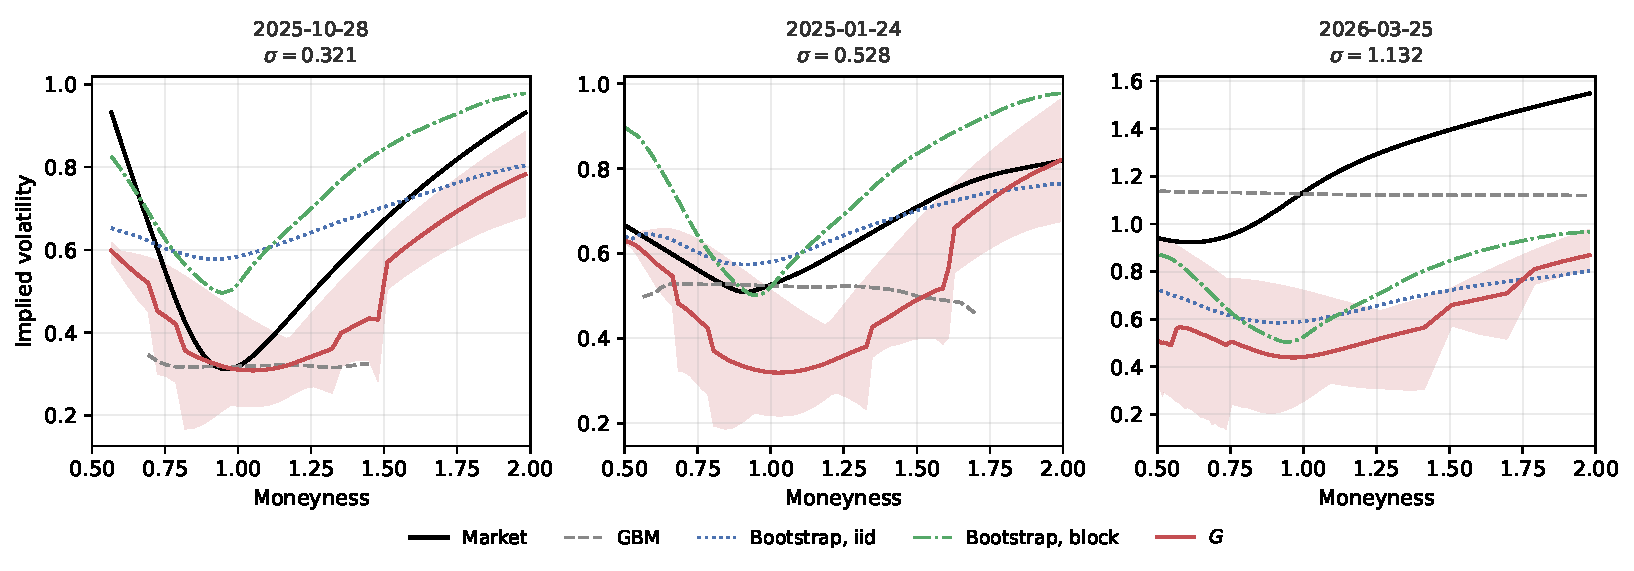
\includegraphics[width=\textwidth]{figures/smiles.pdf}
    \caption{Implied volatility against moneyness on three valuation dates}
    \label{fig:vol-smile-models}
\end{figure}

The market implied volatility is a smile on all three valuation dates. GBM produces a flat implied volatility, since a single $\sigma$ applies to
every strike. Both bootstrap modes overprice the options on the first two valuation dates. The block mode captures the shape of the market, while the $\mathrm{iid}$ mode produces a flatter smile. The implied volatility of $G$ lies below the market on all three dates. 

The third date falls in the 2026 disruption described in Sec.~\ref{sec:gas-markets}. The market implied volatility rises from \num{0.92} for the at-the-money strike to \num{1.55} for the far out-of-the-money strike. Both bootstrap modes and $G$ stay below \num{1.0}. The bootstrap draws from the same training split on every valuation date (Sec.~\ref{sec:benchmarks}), so the simulated distribution does not change with the market conditions. GBM matches the market at the at-the-money strike, since its $\sigma$ is taken from there. $G$ is conditioned on the returns preceding the valuation date. The annualized spread of the simulated \num{20}-day return of $G$ and the block bootstrap is reported in Fig.~\ref{fig:conditioning}, together with the implied volatility at the at-the-money strike.

\begin{figure}[htbp]
    \centering
    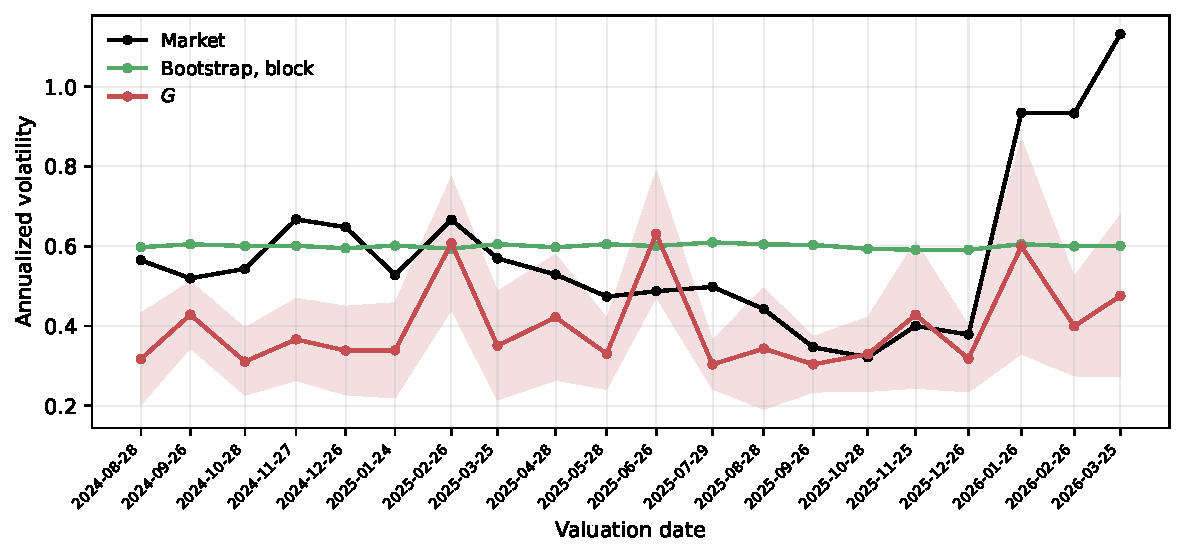
\includegraphics[width=\textwidth]{figures/conditioning.pdf}
    \caption{Annualized volatility on each valuation date}
    \label{fig:conditioning}
\end{figure}

The spread of the block bootstrap ranges from \num{0.588} to \num{0.608}. The spread of $G$ ranges from \num{0.300} to \num{0.615}, and its correlation with the spread of the realized returns in the condition window is \num{0.752}. The simulated distribution of $G$ widens when the preceding returns are turbulent. As a result, the conditioning of $G$ produces a response. The spread of $G$ is below the implied volatility of the market on \num{17} of the \num{20} valuation dates, so the response does not reach the level of the market.

The reported results of $G$ were generated with the ForGAN baseline cost function. The $\mathrm{PnL}^{*}_{a}$ and $\mathrm{PnL}^{*}_{a}$ \& $\mathrm{MSE}$ branches closest to the test split were priced as well (Sec.~\ref{sec:effect-cost}). The results are reported in Tab.~\ref{tab:price-error-branches}. The error of the ForGAN baseline is the lowest among the three cost function branches. The seed spread of the ForGAN baseline is the smallest at \num{0.041} against \num{0.369} for the $\mathrm{PnL}^{*}_{a}$ branch. The signed error of the $\mathrm{PnL}^{*}_{a}$ branch is \num{0.023} with a seed spread of \num{0.508}, so some seeds price above the market and others below. Compared with the ForGAN baseline, the seed spread of the $\mathrm{PnL}^{*}_{a}$ \& $\mathrm{MSE}$ branch is narrower on most of the generated return statistics (Sec.~\ref{sec:effect-cost}) and wider on the option prices.
The seed spread is not explained by the excess kurtosis of the generated returns. In the $\mathrm{PnL}^{*}_{a}$ branch, seed \num{2} has the highest excess kurtosis at \num{21.59} and an error of \num{0.303}, close to the errors of the other seeds. In contrast, seed \num{4} has the largest error of \num{1.101} with an excess kurtosis of \num{11.15}. As a result, the divergence arises in the recursive rollout of the generated returns (Sec.~\ref{sec:pricing-setup}), and not in the one-step distribution

\begin{table}[htbp]
  \centering
  \begin{tabular}{llrrrr}
    \toprule
    Cost function & Seed & Kurtosis & $e$ & $s$ & Inverted (\si{\percent}) \\
    \midrule
    ForGAN & 0 & 13.24 & 0.199 & $-0.163$ & 74.9 \\
           & 1 &  7.61 & 0.237 & $-0.214$ & 96.2 \\
           & 2 & 12.46 & 0.308 & $-0.287$ & 79.1 \\
           & 3 &  9.38 & 0.251 & $-0.200$ & 87.4 \\
           & 4 &  7.93 & 0.279 & $-0.278$ & 61.4 \\
    \addlinespace
    $\mathrm{PnL}^{*}_{a}$ & 0 & 10.12 & 0.193 & $-0.168$ & 92.4 \\
           & 1 &  8.40 & 0.366 & $-0.047$ & 89.3 \\
           & 2 & 21.59 & 0.303 & $-0.303$ & 80.9 \\
           & 3 &  8.90 & 0.284 & $-0.281$ & 83.0 \\
           & 4 & 11.15 & 1.101 & \phantom{$-$}0.912 & 79.0 \\
    \addlinespace
    $\mathrm{PnL}^{*}_{a}$ \& $\mathrm{MSE}$ & 0 & 11.62 & 0.208 & $-0.160$ & 92.2 \\
           & 1 & 11.88 & 0.320 & $-0.313$ & 73.5 \\
           & 2 & 12.30 & 0.230 & $-0.222$ & 93.9 \\
           & 3 &  5.39 & 0.271 & $-0.241$ & 80.4 \\
           & 4 & 12.23 & 0.549 & \phantom{$-$}0.190 & 86.2 \\
    \bottomrule
  \end{tabular}
  \caption{Excess kurtosis of the generated returns and option pricing
           results per seed, configuration 8}
  \label{tab:price-error-branches}
\end{table}

The prices generated by $G$ deviate further from the market than the prices of the benchmarks in every moneyness range. The deviation is a systematic underpricing, and $G$ reaches the fewest strikes. However, $G$ is the only model that responds to the state of the market at the valuation date, although the response does not reach the level of the market.

% \todo{The TTF return
% series studied in this thesis is positively skewed instead, as reported in
% Sec.~\ref{sec:ttf-properties}. Supply disruptions such as those described in
% Sec.~\ref{sec:gasmarkets} raise prices sharply, while no comparable mechanism lowers them.
% The skewness determines the tilt of the volatility smile described in
% Sec.~\ref{sec:options}, and therefore the relative value of calls and puts at equal distance
% from the current price. cite Geman????}